\documentclass[11pt]{article}

% --- Packages ---
\usepackage{amsmath, amssymb, amsthm, mathtools}
\usepackage{geometry}
\usepackage{hyperref}
\usepackage{enumitem}
\usepackage{microtype}
\usepackage{cleveref}
\usepackage{tikz}
\usepackage{pgfplots}
\pgfplotsset{compat=1.17}

\geometry{margin=1in}
\hypersetup{colorlinks=true, linkcolor=blue, citecolor=blue, urlcolor=blue}

% --- Theorem environments ---
\theoremstyle{plain}
\newtheorem{theorem}{Theorem}[section]
\newtheorem{proposition}{Proposition}[section]
\newtheorem{lemma}{Lemma}[section]
\newtheorem{corollary}{Corollary}[section]

\theoremstyle{definition}
\newtheorem{definition}{Definition}[section]
\newtheorem{assumption}{Assumption}[section]

\theoremstyle{remark}
\newtheorem{remark}{Remark}[section]
\newtheorem{example}{Example}[section]

% --- Cleveref names ---
\crefname{theorem}{Theorem}{Theorems}
\crefname{proposition}{Proposition}{Propositions}
\crefname{lemma}{Lemma}{Lemmas}
\crefname{corollary}{Corollary}{Corollaries}
\crefname{definition}{Definition}{Definitions}
\crefname{assumption}{Assumption}{Assumptions}
\crefname{remark}{Remark}{Remarks}
\crefname{example}{Example}{Examples}
\crefname{section}{Section}{Sections}

% --- Commands ---
\newcommand{\R}{\mathbb{R}}
\newcommand{\E}{\mathbb{E}}
\newcommand{\F}{\mathcal{F}}
\newcommand{\K}{\mathcal{K}}
\newcommand{\PP}{\mathbb{P}}
\newcommand{\QQ}{\mathbb{Q}}
\newcommand{\ip}[2]{\langle #1, #2 \rangle}
\newcommand{\norm}[1]{\| #1 \|}
\newcommand{\dGamma}{\Delta\Gamma}
\newcommand{\bracket}[1]{\langle #1 \rangle}
\DeclareMathOperator{\Cov}{Cov}
\DeclareMathOperator{\Var}{Var}
\DeclareMathOperator{\Dom}{Dom}

\title{Risk-Neutral Pricing with Memory:\\[0.3em]
Volterra Constraints and Operator-Induced Drift}
\author{Ramiro Fontes\\[0.5em]
\small Quijotic Research\\[0.3em]
\small\texttt{ramirofontes@gmail.com}}
\date{February 2026}

\begin{document}
\maketitle

\begin{abstract}
Classical risk-neutral pricing assumes that the market price of risk satisfies
a pointwise algebraic constraint: drift cancellation is instantaneous. When
asset dynamics include memory---driven by Volterra-type operators
$Z_t = \int_0^t K(t,s)\,dM_s$ where $M$ is a martingale driver and $K$ a
causal kernel---this picture breaks down. The risk-neutral constraint becomes
a \emph{Volterra integral equation}, not a pointwise relation.

This paper characterizes risk-neutral measures when dynamics have memory.
The main results are:

\begin{enumerate}[label=(\roman*)]
\item \textbf{Operator-induced drift} (\Cref{thm:girsanov-main}): Under measure
change from $\PP$ to an equivalent measure $\QQ$, each Volterra observable $Z$
acquires a drift that depends on the full history through the kernel $K$, not
just instantaneous volatility.

\item \textbf{Risk-neutral constraint as Volterra equation} (\Cref{cor:rn-constraint}):
For tradables driven by memory factors, the discounted-martingale condition
becomes an integral equation for the market price of risk $\theta$---the
\emph{Volterra risk-neutral constraint} (VRNC). Risk-neutrality is equivalent
to \emph{annihilating the memory contribution to expected returns}.

\item \textbf{Bracket invariance} (\Cref{thm:girsanov-main}): The quadratic
variation $\bracket{M}$ of the driver is unchanged under equivalent measure
changes. Consequently, Hurst exponents (roughness parameters), and other
bracket-derived quantities are representation invariants.

\item \textbf{Hedging density under the risk-neutral measure} (\Cref{thm:clark-ocone-Q}):
The replicating strategy is computable via an operator calculus (the modified
Leibniz rule) and Bayes' formula.
\end{enumerate}

The measure-change formula itself is classical (Girsanov); what is new is the
characterization of risk-neutrality as an operator constraint when dynamics
include memory. This clarifies why calibration in rough volatility models
often succeeds while hedging fails: the two tasks impose different constraints,
and only the Volterra formulation captures both.

\medskip
\noindent\textbf{MSC 2020:} 60H07, 60H30, 60G44, 91G20.

\noindent\textbf{Keywords:} Risk-neutral pricing; Volterra processes; memory;
operator derivative; market price of risk; rough volatility.
\end{abstract}

\tableofcontents

%==============================================================================
\section{Introduction}\label{sec:intro}
%==============================================================================

\subsection{Motivation}

In classical asset pricing, the risk-neutral constraint is pointwise: if
$dS/S = \mu\,dt + \sigma\,dW$, then the market price of risk $\theta = (\mu - r)/\sigma$
cancels drift instantaneously. This works because the dynamics are Markovian---the
future depends on the present only through the current state.

When dynamics include memory, this picture breaks down. Consider an asset driven
by both fresh noise and a memory factor:
\[
\frac{dS}{S} = \mu\,dt + \lambda\,dM + \beta\,dZ, \quad
Z_t = \int_0^t K(t,s)\,dM_s.
\]
The memory term $Z$ aggregates past innovations through the kernel $K$. A
measure change that tilts $M$ affects $Z$ through the \emph{entire history}
of the kernel weights, not just the instantaneous volatility. The risk-neutral
constraint becomes a Volterra integral equation, not an algebraic relation.

This paper characterizes risk-neutral measures for such dynamics. The measure-change
formula itself is classical (Girsanov for continuous martingales); what is new
is the identification of the risk-neutral constraint as an operator equation
and the consequences this has for pricing and hedging in markets with memory.

In contrast to classical Markovian models where risk-neutrality is enforced
pointwise via drift cancellation, the present framework yields integral
(Volterra-type) constraints reflecting the underlying memory structure.

\subsection{Main results}

We establish four principal results. (Notation: $M$ is a continuous martingale
driver, $\bracket{M}$ its quadratic variation, $K$ a causal kernel,
$Z_t = \int_0^t K(t,s)\,dM_s$ the Volterra observable, and $\dGamma(t,h)$ the
fresh-noise energy increment. Precise definitions are in \Cref{sec:framework}.)

\begin{enumerate}[label=(\arabic*)]
\item \textbf{Measure change and operator-induced drift} (\Cref{thm:girsanov-main}).
Let $\theta$ be predictable with appropriate integrability, and let $\QQ$ be
the equivalent measure defined by the Dol\'eans exponential (stochastic exponential)
$L_T = \mathcal{E}(-\int_0^T \theta_s\,dM_s)$. Then:
\begin{itemize}
\item The tilted driver $M_t^{\QQ} := M_t + \int_0^t \theta_s\,d\bracket{M}_s$
is a $\QQ$-martingale with $\bracket{M^{\QQ}} = \bracket{M}$.
\item The Volterra observable decomposes as $Z_t = Z_t^{\QQ} + B_t^\theta$, where
$Z_t^{\QQ} = \int_0^t K(t,s)\,dM_s^{\QQ}$ and the \emph{operator-induced drift} is
$B_t^\theta = -\int_0^t K(t,s)\theta_s\,d\bracket{M}_s$.
\item The fresh-noise energy is invariant: $\dGamma^{\QQ}(t,h) = \dGamma^{\PP}(t,h)$.
\end{itemize}

\item \textbf{Multi-dimensional extension} (\Cref{thm:girsanov-vector}).
For vector drivers $M \in \R^d$ and multiple kernels $K^{(a)}$, the bracket
matrix $\bracket{M}$ is preserved, and each observable acquires an
operator-induced drift $B^{(a),\theta} = -K^{(a)}[d\bracket{M}\,\theta]$.

\item \textbf{Volterra risk-neutral constraint (VRNC)} (\Cref{cor:rn-constraint}).
For a tradable with dynamics driven by both fresh noise and memory factors,
the discounted-martingale condition becomes a Volterra integral equation for $\theta$.
The market price of risk is determined by the full kernel structure, not pointwise.

\item \textbf{Hedging density under the risk-neutral measure} (\Cref{thm:clark-ocone-Q}).
A square-integrable $\QQ$-claim $F$ admits a martingale representation
$F = \E^{\QQ}[F] + \int_0^T \phi_t^\top\,dM_t^{\QQ}$, where the hedging
density $\phi_t$ is computable via Bayes' formula and the modified Leibniz
rule (the corrected product rule for operator derivatives; see \Cref{sec:density}).
\end{enumerate}

\subsection{Significance}

The Volterra risk-neutral constraint (VRNC, \Cref{cor:rn-constraint}) is the
conceptual core of this paper. It shows that in markets with memory, the market
price of risk $\theta$ cannot be read off pointwise from asset dynamics---it must
be solved for as an integral equation determined by the kernel structure.

The bracket invariance result (\Cref{thm:girsanov-main}(3)) explains why:
any model feature built purely from the kernel family $K$ and the driver
bracket $d\bracket{M}$ is unchanged across equivalent measures. This includes:

\begin{itemize}
\item The fresh-noise energy increment $\dGamma(t,h)$.
\item Any Hurst exponent extracted from the scaling $\dGamma(t,h) \asymp h^{2H}$.
\item Roughness diagnostics and regime classifications.
\item Marginal distributions of increments (up to drift).
\end{itemize}

In short: \emph{the geometry is objective; only the drift is subjective}.

This separation has practical consequences. Calibration to option prices
targets marginal distributions---which are bracket-determined, hence
measure-invariant. Hedging targets conditional expectations---which depend
on the drift, hence on the full Volterra constraint. Classical pointwise
intuition conflates these; the operator formulation separates them. This
explains why calibration in rough volatility models often succeeds while
hedging remains problematic: the two tasks impose structurally different
constraints.

\subsection{Related work}

The operator factorization framework was developed in \cite{Fontes2026a},
with extensions to fractional processes \cite{Fontes2026b}, non-semimartingale
It\^o formulas \cite{Fontes2026c}, and kernel-level geometry \cite{Fontes2026f}.
The bracket-corrected calculus of \cite{Fontes2026g} provides the modified
Leibniz rule---the corrected product rule $D_M(FG) = \E[F|\F_t]\,D_M G + \E[G|\F_t]\,D_M F$
for operator derivatives---used here for density calculations.

For classical Girsanov theory, see \cite{KaratzasShreve1991}. The rough
volatility literature \cite{GatheralJaissonRosenbaum2018} motivates the
need for measure change theory beyond semimartingales. Volterra processes
and their stochastic calculus are treated in \cite{Decreusefond1999} and
the rough path literature \cite{FrizHairer2014}.

\subsection{Contribution and scope}

The measure-change formula for continuous martingales is classical
\cite{KaratzasShreve1991, JacodShiryaev2003}; this paper does not claim
a new Girsanov theorem or a new existence result for equivalent martingale
measures. Rather, we characterize the risk-neutral constraint when asset
dynamics include operator-driven memory terms:

\begin{enumerate}[label=(\roman*)]
\item \textbf{The Volterra risk-neutral constraint (VRNC)} (\Cref{cor:rn-constraint}).
Classical theory gives a pointwise algebraic equation for $\theta$. In the
presence of memory, this becomes a Volterra integral equation---risk-neutrality
requires annihilating the memory contribution to expected returns, not just
matching instantaneous drift.

\item \textbf{Operator-induced drift structure} (\Cref{thm:girsanov-main}).
The drift acquired by a Volterra observable under measure change is
$B^\theta = -K[\theta \cdot d\bracket{M}]$, determined by the kernel geometry.
This is not a pointwise correction but a history-dependent functional.

\item \textbf{Bracket invariance} (\Cref{thm:girsanov-main}(3)).
Fresh-noise energy, Hurst exponents, and roughness diagnostics are unchanged
under equivalent measure changes. These are geometric properties of the kernel,
not probabilistic artifacts of the reference measure.

\item \textbf{Hedging under the risk-neutral measure} (\Cref{thm:clark-ocone-Q}).
The replicating strategy is computable via Bayes' formula and the modified
Leibniz rule \cite{Fontes2026g}, connecting pricing to the operator calculus.
\end{enumerate}

\subsection{Organization}

\Cref{sec:framework} recalls the Volterra framework and fixes notation.
\Cref{sec:girsanov} establishes measure change with bracket invariance.
\Cref{sec:vector} extends to vector drivers and multiple kernels.
\Cref{sec:finance} derives the risk-neutral constraint as a Volterra equation.
\Cref{sec:density} develops density differentiation and Bayes' rule for
operator derivatives. \Cref{sec:clark-ocone} proves the Clark--Ocone--type
representation under $\QQ$ and derives the hedging recipe. \Cref{sec:examples} works concrete examples.
\Cref{sec:limitations} states scope limitations.

%==============================================================================
\section{Framework}\label{sec:framework}
%==============================================================================

We recall the Volterra framework from \cite{Fontes2026f}, specialized to the
setting needed for measure change theory.

\subsection{Probabilistic setup}

Let $(\Omega, \F, (\F_t)_{t \in [0,T]}, \PP)$ be a filtered probability space
satisfying the usual conditions. Let $M$ be a continuous square-integrable
$\PP$-martingale with $M_0 = 0$ and predictable quadratic variation
$\bracket{M}$. Throughout, we assume $M$ possesses the \emph{predictable
representation property}: every $F \in L^2(\F_T, \PP)$ admits a representation
$F = \E[F] + \int_0^T \phi_t\,dM_t$ for some predictable $\phi$. The operator
derivative $D_M$ (\Cref{def:DM}) is then the Hilbert-space adjoint of
stochastic integration with respect to $M$, yielding a Clark--Ocone--type
representation by construction (see \Cref{prop:clark-ocone-P} and
\Cref{rem:clark-ocone-distinction}).

Define the bracket measure
\[
\mu(ds) := d\bracket{M}_s.
\]

\begin{assumption}[Driver regularity]\label{ass:driver}
The bracket process $\bracket{M}$ is absolutely continuous with respect to
Lebesgue measure: $d\bracket{M}_t = a_t\,dt$ for some predictable process
$a_t \ge 0$. We write $\mu(ds) = a_s\,ds$.
\end{assumption}

\Cref{ass:driver} simplifies exposition but is not essential; results extend
to general continuous martingales with minor modifications.

\subsection{Volterra observables}

\begin{definition}[Volterra observable]\label{def:volterra}
A \emph{causal kernel} is a measurable function $K : [0,T]^2 \to \R$ with
$K(t,s) = 0$ for $s > t$. The associated \emph{Volterra observable} is
\[
Z_t := \int_0^t K(t,s)\,dM_s.
\]
\end{definition}

\begin{assumption}[Kernel integrability]\label{ass:kernel}
The kernel $K$ satisfies
\[
\sup_{t \in [0,T]} \int_0^t K(t,s)^2\,\mu(ds) < \infty.
\]
\end{assumption}

Under \Cref{ass:kernel}, $Z_t$ is well-defined and square-integrable by the
It\^o isometry. Importantly, no semimartingale assumption is imposed on the
observable $Z$; for singular kernels (e.g.\ $K(t,s) = (t-s)^{H-1/2}$ with
$H < 1/2$), $Z$ is typically \emph{not} a semimartingale. All
measure-change effects in this paper are carried by the driver $M$, not
the observables.

\subsection{Fresh-noise energy}

\begin{definition}[Fresh-noise energy increment]\label{def:DeltaGamma}
For $t \in [0,T)$ and $h > 0$ with $t + h \le T$, define
\[
\dGamma(t,h) := \int_t^{t+h} K(t+h,s)^2\,\mu(ds).
\]
\end{definition}

The increment $\dGamma(t,h)$ measures the energy contributed by innovations
on $(t, t+h]$. It is the fundamental second-order object of the Volterra
framework, governing It\^o corrections and determining Hurst scaling
\cite{Fontes2026f}.

\subsection{The operator derivative}

\begin{definition}[Operator derivative]\label{def:DM}
Let $F \in L^2(\F_T, \PP)$. The \emph{operator derivative} $D_M F$ is the
unique element of $L^2(\Omega \times [0,T],\, d\bracket{M} \otimes d\PP)$ satisfying
\begin{equation}\label{eq:DM-riesz}
\E\!\left[F \int_0^T \varphi_t\,dM_t\right]
= \E\!\left[\int_0^T (D_M F)_t\,\varphi_t\,d\bracket{M}_t\right]
\end{equation}
for all predictable $\varphi$ with $\E\int_0^T \varphi_t^2\,d\bracket{M}_t < \infty$.
\end{definition}

Existence and uniqueness follow from the Riesz representation theorem applied
to the continuous linear functional
$\varphi \mapsto \E[F \int_0^T \varphi_t\,dM_t]$ on $L^2(d\bracket{M} \otimes d\PP)$.
This is the specialization of the general operator derivative \cite{Fontes2026d}
to the continuous martingale energy space $H_M = L^2(\Omega \times [0,T],\, d\bracket{M} \otimes d\PP)$.
For comparison with the classical Malliavin derivative, see \cite{Nualart2006}.
When the filtration is generated by $M$, the martingale representation
$F = \E[F] + \int_0^T \phi_s\,dM_s$ gives the explicit identification
$(D_M F)_t = \phi_t$.

\begin{remark}[Connection to predictable representation]\label{rem:connection-rep}
Under the standing assumption that $M$ possesses the predictable representation
property, the operator derivative $(D_M F)_t$ coincides with the unique predictable
integrand in the Galtchouk--Kunita--Watanabe decomposition of $F$ with respect to $M$.
The mathematical content is classical; the operator formulation packages it as an
adjoint/Riesz representer, making the algebraic structure---particularly the
measure-invariance of the bracket---explicit. This organization is essential for
the Girsanov theory developed in \Cref{sec:girsanov}.
\end{remark}

\begin{remark}[No limit required]\label{rem:no-epsilon}
The definition \eqref{eq:DM-riesz} is purely algebraic---it involves no
$\epsilon \to 0$ limits, no time-local increments, and no regularity
assumptions beyond square integrability. This is deliberate: since Girsanov
preserves $\bracket{M}$, the operator derivative is the natural invariant
object under measure change. When $\bracket{M}$ has Lebesgue density $a_t > 0$,
one recovers the conditional increment formula
\[
(D_M F)_t = a_t^{-1}\lim_{\epsilon \downarrow 0} \epsilon^{-1}\,
\E[F(M_{t+\epsilon} - M_t) \mid \F_t]
\]
as a consequence, not a definition \cite{Fontes2026g}.
\end{remark}

\begin{remark}[Domain and boundedness]\label{rem:domain}
Under the predictable representation property, $D_M$ is everywhere-defined on
$L^2(\F_T)$: every $F \in L^2(\F_T)$ admits a unique martingale representation,
hence a unique operator derivative. However, $D_M$ is unbounded as a map
$L^2(\Omega) \to L^2(\Omega \times [0,T], d\bracket{M} \otimes d\PP)$. The
energy norm $\|D_M F\|_{H_M}^2 = \Var(F)$ by It\^o isometry, so $D_M$ is
bounded on no proper dense subspace. Closedness of $\delta_M$ suffices for
existence of the Riesz representer; no additional functional-analytic machinery
is required.
\end{remark}

\subsection{The operator factorization}

The operator derivative is not an arbitrary differentiation---it is the
exact inverse (modulo expectation) of stochastic integration.

\begin{proposition}[Adjoint martingale representation {\cite{Fontes2026a}}]\label{prop:clark-ocone-P}
Let $F \in L^2(\F_T, \PP)$. Under the standing assumption that $M$
possesses the predictable representation property, we have
\begin{equation}\label{eq:factorization}
(\mathrm{Id} - \E)\,F = \delta_M(D_M F),
\end{equation}
where $\delta_M(\varphi) := \int_0^T \varphi_t\,dM_t$ denotes stochastic
integration against $M$. Equivalently,
\[
F = \E[F] + \int_0^T (D_M F)_t\,dM_t.
\]
\end{proposition}

\begin{remark}[Relationship to Clark--Ocone]\label{rem:clark-ocone-distinction}
On Wiener space, \Cref{prop:clark-ocone-P} reduces to the classical
Clark--Ocone formula. In the present setting, it holds for general continuous
martingale drivers and is derived via Riesz representation rather than
Malliavin calculus. No Gaussian structure, chaos expansion, or pathwise
derivative is used. We refer to this as a \emph{Clark--Ocone--type}
representation to signal the structural parallel without implying
dependence on the Malliavin framework.
\end{remark}

This identity---purely a consequence of the Riesz definition and
martingale representation---is the reason the operator derivative is the
correct density for hedging and representation. Its algebraic form
$(\mathrm{Id} - \E) = \delta_M \circ D_M$ is measure-agnostic: under
$\QQ$, it becomes $(\mathrm{Id} - \E^{\QQ})\,F = \delta_{M^{\QQ}}(D_{M^{\QQ}} F)$
with the same structure, because Girsanov preserves the bracket and hence
the adjoint pair $(D_M, \delta_M)$.

%==============================================================================
\section{Measure Change and Bracket Invariance}\label{sec:girsanov}
%==============================================================================

\subsection{Setup}

Let $\theta$ be a predictable $\R$-valued process satisfying the integrability
condition
\begin{equation}\label{eq:theta-int}
\int_0^T \theta_s^2\,d\bracket{M}_s < \infty \quad \text{a.s.}
\end{equation}

Define the Dol\'eans exponential (stochastic exponential)
\begin{equation}\label{eq:doleans}
L_t := \mathcal{E}\left(-\int_0^t \theta_s\,dM_s\right)
:= \exp\left(-\int_0^t \theta_s\,dM_s - \frac{1}{2}\int_0^t \theta_s^2\,d\bracket{M}_s\right).
\end{equation}

\begin{assumption}[Martingale property]\label{ass:novikov}
The process $L$ is a true $\PP$-martingale. (This holds, e.g., under the
Novikov condition $\E[\exp(\frac{1}{2}\int_0^T \theta_s^2\,d\bracket{M}_s)] < \infty$.)
\end{assumption}

Under \Cref{ass:novikov}, we define the equivalent measure $\QQ$ by
\begin{equation}\label{eq:Q-def}
\frac{d\QQ}{d\PP}\bigg|_{\F_T} = L_T.
\end{equation}

\subsection{Main theorem}

\begin{theorem}[Measure change with bracket invariance]\label{thm:girsanov-main}
Under \Cref{ass:driver,ass:kernel,ass:novikov}, the following hold:

\begin{enumerate}[label=(\arabic*)]
\item \textbf{Driver-level Girsanov.} The process
\begin{equation}\label{eq:MQ-def}
M_t^{\QQ} := M_t + \int_0^t \theta_s\,d\bracket{M}_s
\end{equation}
is a continuous $\QQ$-martingale with
\begin{equation}\label{eq:bracket-preserved}
\bracket{M^{\QQ}}_t = \bracket{M}_t.
\end{equation}

\item \textbf{Operator pushforward decomposition.} The Volterra observable
$Z$ admits the exact decomposition
\begin{equation}\label{eq:Z-decomp}
Z_t = Z_t^{\QQ} + B_t^\theta,
\end{equation}
where
\begin{align}
Z_t^{\QQ} &:= \int_0^t K(t,s)\,dM_s^{\QQ}, \label{eq:ZQ-def} \\
B_t^\theta &:= -\int_0^t K(t,s)\,\theta_s\,d\bracket{M}_s. \label{eq:Btheta-def}
\end{align}
Under $\QQ$, the noise part $Z^{\QQ}$ is the same operator applied to a
martingale; the measure change induces the deterministic operator-valued
drift $B^\theta$.

\item \textbf{Bracket invariance.} For all admissible $t, h$,
\begin{equation}\label{eq:DG-invariance}
\dGamma^{\QQ}(t,h) := \int_t^{t+h} K(t+h,s)^2\,d\bracket{M^{\QQ}}_s
= \int_t^{t+h} K(t+h,s)^2\,d\bracket{M}_s = \dGamma^{\PP}(t,h).
\end{equation}
\end{enumerate}
\end{theorem}

\begin{proof}
\textbf{Part (1):} This is the classical continuous-martingale Girsanov theorem
applied at the driver level. Under \Cref{ass:novikov}, the process $L$ is a
true martingale, so $M^{\QQ}$ defined by \eqref{eq:MQ-def} is a $\QQ$-local
martingale. The bracket preservation \eqref{eq:bracket-preserved} follows
because $M^{\QQ}$ differs from $M$ by a finite-variation process:
\[
\bracket{M^{\QQ}}_t = \bracket{M + \int_0^\cdot \theta_s\,d\bracket{M}_s}_t
= \bracket{M}_t,
\]
since quadratic variation ignores finite-variation perturbations.

\textbf{Part (2):} From \eqref{eq:MQ-def}, we have
$dM_s = dM_s^{\QQ} - \theta_s\,d\bracket{M}_s$. Substituting into the
definition of $Z_t$:
\begin{align*}
Z_t &= \int_0^t K(t,s)\,dM_s \\
&= \int_0^t K(t,s)\,dM_s^{\QQ} - \int_0^t K(t,s)\,\theta_s\,d\bracket{M}_s \\
&= Z_t^{\QQ} + B_t^\theta.
\end{align*}
The first integral is a stochastic integral against the $\QQ$-martingale
$M^{\QQ}$; the second is a Lebesgue--Stieltjes integral in $s$ for each
fixed $t$, hence a deterministic, non-martingale correction. This
decomposition is exact and requires no semimartingale assumption on $Z$.

\textbf{Part (3):} The fresh-noise energy is defined purely in terms of
$K$ and $d\bracket{M}$. Since $\bracket{M^{\QQ}} = \bracket{M}$ by part (1),
the equality \eqref{eq:DG-invariance} follows immediately.
\end{proof}

\begin{remark}[No semimartingale assumption on $Z$]
The decomposition \eqref{eq:Z-decomp} holds for any Volterra observable,
including fractional Brownian motion and rough processes. The measure change
is performed where it belongs---on the driver $M$---and the effect on $Z$
is induced by the operator structure.
\end{remark}

\begin{remark}[Non-Gaussian drivers]\label{rem:non-gaussian}
The construction applies to any continuous martingale driver $M$, not only
Brownian motion. In particular, it accommodates:
\begin{itemize}
\item Time-changed Brownian drivers $M_t = W_{\tau_t}$ with random time change $\tau$,
\item Stochastic volatility drivers $M_t = \int_0^t \sigma_s\,dW_s$ where $\sigma$ is
itself a stochastic process,
\item Other continuous martingale drivers arising from filtration enlargement or
market microstructure models.
\end{itemize}
The observable processes may be non-Markovian and need not be
semimartingales. The Girsanov formula in exponential form \eqref{eq:doleans}
is most natural for continuous martingales; extensions to jump drivers (L\'evy,
Poisson) require the jump-compensator version of Girsanov, but the same
``driver-level then operator pushforward'' philosophy carries over.
\end{remark}

\begin{remark}[Recovery of classical Girsanov when $K = \mathbf{1}$]\label{rem:classical-recovery}
When $K(t,s) = \mathbf{1}_{\{s \le t\}}$, the observable equals the driver:
$Z_t = M_t$. The drift functional reduces to
$B_t^\theta = -\int_0^t \theta_s\,d\bracket{M}_s$, and the decomposition
\eqref{eq:Z-decomp} becomes the classical Girsanov identity
$M_t = M_t^{\QQ} - \int_0^t \theta_s\,d\bracket{M}_s$. The operator framework
thus strictly generalizes classical measure change theory: non-trivial kernels
yield non-trivial (history-dependent) drift functionals, while the Markov
kernel recovers the standard result.
\end{remark}

\begin{remark}[Interpretation of bracket invariance]
\Cref{thm:girsanov-main}(3) asserts that $\dGamma$ is a \emph{geometric}
quantity, not a probabilistic one. Any scaling law extracted from
$\dGamma(t,h) \asymp h^{2H}$ is invariant under equivalent measure changes.
The Hurst parameter is an intrinsic property of the representation $(K, \mu)$,
observable under any equivalent measure.
\end{remark}

\subsection{The drift functional}

The operator-valued drift $B^\theta$ deserves separate attention.

\begin{definition}[Operator drift functional]\label{def:drift-functional}
For a predictable process $\theta$, define the \emph{$K$-drift functional}
\begin{equation}\label{eq:drift-functional}
B_t^\theta := -(K[\theta \cdot d\bracket{M}])_t := -\int_0^t K(t,s)\,\theta_s\,d\bracket{M}_s.
\end{equation}
\end{definition}

\begin{proposition}[Properties of the drift functional]\label{prop:drift-properties}
The drift functional $B^\theta$ satisfies:
\begin{enumerate}[label=(\alph*)]
\item \textbf{Causality:} $B_t^\theta$ depends only on $\{(\theta_s, d\bracket{M}_s) : s \le t\}$.
\item \textbf{Linearity:} $B^{\alpha\theta_1 + \beta\theta_2} = \alpha B^{\theta_1} + \beta B^{\theta_2}$.
\item \textbf{History dependence:} Even if $\theta$ is constant, $B_t^\theta$
depends on the full history $\{K(t,s) : s \le t\}$.
\item \textbf{Deterministic and non-martingale:} For each $t$, $B_t^\theta$
is a deterministic functional of $(\theta, K, d\bracket{M})$; it carries no
martingale component. When $t \mapsto K(t,\cdot)$ is sufficiently regular
(e.g.\ smooth or exponential kernels), the path $t \mapsto B_t^\theta$ has
finite variation. For singular kernels (e.g.\ $K(t,s) = (t-s)^{H-1/2}$,
$H < 1/2$), $B^\theta$ may fail to be of bounded variation in $t$.
\end{enumerate}
\end{proposition}

\begin{proof}
Properties (a)--(c) are immediate from the definition. For (d),
under \Cref{ass:driver}, $B_t^\theta = -\int_0^t K(t,s)\,\theta_s\,a_s\,ds$
is a Lebesgue integral in $s$ for each $t$, hence a deterministic,
non-martingale correction. Regularity in $t$ depends on the kernel:
for kernels with $t \mapsto K(t,\cdot)$ absolutely continuous in
$L^2(\mu)$, the path $t \mapsto B_t^\theta$ has finite variation;
for singular kernels this may fail.
\end{proof}

%==============================================================================
\section{Vector Drivers and Multiple Kernels}\label{sec:vector}
%==============================================================================

We extend to the setting relevant for multi-factor models.

\subsection{Setup}

Let $M = (M^1, \ldots, M^d)$ be a continuous $d$-dimensional $\PP$-local
martingale with predictable bracket matrix
\[
\bracket{M}_t = \big(\bracket{M^i, M^j}_t\big)_{i,j=1}^d.
\]
Write $d\bracket{M}_t$ for the matrix-valued measure.

Fix $m$ causal kernels $K^{(a)} : [0,T]^2 \to \R^d$ (row vectors), $a = 1, \ldots, m$,
and define observables
\[
Z_t^{(a)} := \int_0^t K^{(a)}(t,s)\,dM_s = \sum_{i=1}^d \int_0^t K^{(a)}_i(t,s)\,dM_s^i.
\]

Define the fresh-noise energy for each $a$:
\[
\dGamma^{(a)}(t,h) := \int_t^{t+h} K^{(a)}(t+h,s)\,d\bracket{M}_s\,K^{(a)}(t+h,s)^\top.
\]

\subsection{Vector measure change}

Let $\theta$ be a predictable $\R^d$-valued process with
$\int_0^T \theta_s^\top\,d\bracket{M}_s\,\theta_s < \infty$ a.s., and assume
the Dol\'eans exponential
\[
L_t := \mathcal{E}\left(-\int_0^t \theta_s^\top\,dM_s\right)
\]
is a true martingale. Define $\QQ$ by $\frac{d\QQ}{d\PP}|_{\F_T} = L_T$.

\begin{theorem}[Vector Girsanov with bracket invariance]\label{thm:girsanov-vector}
Under the above assumptions:

\begin{enumerate}[label=(\arabic*)]
\item \textbf{Vector driver shift.} The process
\[
M_t^{\QQ} := M_t + \int_0^t d\bracket{M}_s\,\theta_s
\]
is a continuous $\QQ$-local martingale with
\[
\bracket{M^{\QQ}}_t = \bracket{M}_t \quad \text{(same bracket matrix)}.
\]

\item \textbf{Multi-kernel pushforward.} For each $a \in \{1, \ldots, m\}$,
\begin{equation}\label{eq:Za-decomp}
Z_t^{(a)} = Z_t^{(a),\QQ} + B_t^{(a),\theta},
\end{equation}
where
\begin{align*}
Z_t^{(a),\QQ} &:= \int_0^t K^{(a)}(t,s)\,dM_s^{\QQ}, \\
B_t^{(a),\theta} &:= -\int_0^t K^{(a)}(t,s)\,d\bracket{M}_s\,\theta_s.
\end{align*}

\item \textbf{Energy invariance.} For each $a$ and admissible $t, h$,
\[
\dGamma^{(a),\QQ}(t,h) = \dGamma^{(a),\PP}(t,h).
\]
\end{enumerate}
\end{theorem}

\begin{proof}
The proof follows the same structure as \Cref{thm:girsanov-main}, with
matrix/vector notation throughout.
\end{proof}

\begin{corollary}[Measure-change invariants]\label{cor:invariants}
Any model feature built purely from the kernel family $\{K^{(a)}\}$ and
the driver bracket $d\bracket{M}$ is invariant across the equivalent
measures generated by exponentials of $\int \theta^\top\,dM$. This includes:
\begin{enumerate}[label=(\alph*)]
\item Fresh-noise energy increments $\dGamma^{(a)}(t,h)$.
\item Hurst/roughness exponents extracted from $\dGamma$ scaling.
\item Cross-kernel correlations $\Gamma_{K^{(a)}, K^{(b)}}$.
\item The ``fresh vs.\ history'' decomposition structure.
\end{enumerate}
\end{corollary}

%==============================================================================
\section{Risk-Neutral Pricing}\label{sec:finance}
%==============================================================================

We derive the risk-neutral constraint for markets driven by memory factors.

\subsection{Asset dynamics}

Consider a tradable $S$ with discounted dynamics
\begin{equation}\label{eq:S-dynamics}
\frac{dS_t}{S_t} = r_t\,dt + \sum_{a=1}^m \beta_t^{(a)}\,dZ_t^{(a)} + \lambda_t^\top\,dM_t,
\end{equation}
where:
\begin{itemize}
\item $r_t$ is the instantaneous interest rate,
\item $\beta^{(a)}$ are predictable loadings on memory factors $Z^{(a)}$,
\item $\lambda_t \in \R^d$ is the loading on fresh noise $dM_t$.
\end{itemize}
Here $dZ_t^{(a)}$ denotes the increment $Z_{t+dt}^{(a)} - Z_t^{(a)}$; since $Z^{(a)}$
may not be a semimartingale, this notation represents the integrated dynamics.

\subsection{The risk-neutral constraint}

\begin{corollary}[Volterra risk-neutral constraint (VRNC)]\label{cor:rn-constraint}
Under the measure $\QQ$ defined by market price of risk $\theta \in \R^d$, the
non-martingale correction to the dynamics relative to $r_t\,dt$ equals
\[
-\lambda_t^\top\,A_t\,\theta_t\,dt + \sum_{a=1}^m \beta_t^{(a)}\,dB_t^{(a),\theta},
\]
where $A_t := d\bracket{M}_t/dt$ is the instantaneous covariance matrix
(guaranteed to exist by \Cref{ass:driver} in the vector setting).
Hence a risk-neutral measure (discounted $S$ a $\QQ$-local martingale) is
obtained by choosing $\theta$ such that, $dt$-a.e.,
\begin{equation}\label{eq:rn-constraint}
\lambda_t^\top\,A_t\,\theta_t - \sum_{a=1}^m \beta_t^{(a)}\,\frac{dB_t^{(a),\theta}}{dt} = 0.
\end{equation}
Here $dB^{(a),\theta}/dt$ denotes the Radon--Nikodym derivative of the drift
functional with respect to Lebesgue measure; when the kernels are regular,
this is simply the time derivative of $B_t^{(a),\theta}$.
When $K$ is singular (e.g.\ fractional kernels), the derivative is understood
distributionally or as a Radon--Nikodym density, and need not exist classically
even though $B^{(a),\theta}$ itself is well-defined as a Volterra integral.
(Under \Cref{ass:driver}; otherwise replace $dt$ by $d\bracket{M}_t$ and
interpret $dB$ as a signed measure in bracket time.)
\end{corollary}

In financial applications, an equivalent measure $\QQ$ under which discounted
asset prices are local martingales is referred to as a \emph{risk-neutral}
(or pricing) measure. In the present setting, the condition
\eqref{eq:rn-constraint} characterizes such a measure when asset dynamics
involve operator-driven, non-Markovian factors.

\begin{proof}
Under $\QQ$, applying the decomposition \eqref{eq:Za-decomp} to the
integrated dynamics \eqref{eq:S-dynamics}, we obtain
\begin{align*}
\frac{dS_t}{S_t} &= r_t\,dt + \sum_{a=1}^m \beta_t^{(a)}\,(dZ_t^{(a),\QQ} + dB_t^{(a),\theta})
+ \lambda_t^\top\,(dM_t^{\QQ} - A_t\,\theta_t\,dt) \\
&= r_t\,dt + \sum_{a=1}^m \beta_t^{(a)}\,dZ_t^{(a),\QQ} + \lambda_t^\top\,dM_t^{\QQ} \\
&\quad - \lambda_t^\top\,A_t\,\theta_t\,dt + \sum_{a=1}^m \beta_t^{(a)}\,dB_t^{(a),\theta}.
\end{align*}
For discounted $S$ to be a $\QQ$-local martingale, the $dt$-terms
must cancel, yielding \eqref{eq:rn-constraint}.
\end{proof}

\begin{remark}[The constraint is a Volterra equation]
Writing out $dB^{(a),\theta}/dt = -\frac{d}{dt}\int_0^t K^{(a)}(t,s)\,A_s\,\theta_s\,ds$
(cf.\ \Cref{def:drift-functional}), the constraint \eqref{eq:rn-constraint} becomes
\[
\lambda_t^\top\,A_t\,\theta_t + \sum_{a=1}^m \beta_t^{(a)}\,\frac{d}{dt}\int_0^t K^{(a)}(t,s)\,A_s\,\theta_s\,ds = 0.
\]
This is a Volterra-type constraint for $\theta$, coupling the current value
$\theta_t$ to the entire history $\{\theta_s : s < t\}$ through the kernels
$K^{(a)}$. When $K$ is singular (e.g.\ fractional kernels with $H < \frac{1}{2}$),
$dB/dt$ is understood as a Radon--Nikodym derivative, and the boundary term
$K(t,t)\,A_t\,\theta_t$ from Leibniz differentiation is absorbed into that notion.
Throughout this paper, all differentiation of Volterra terms is understood in the
weak or Radon--Nikodym sense; no pointwise differentiability of $K$ is assumed.
In discrete time, the constraint becomes a lower-triangular linear system.
\end{remark}

\begin{remark}[Interpretation]
The market price of risk in memory markets is \emph{history-priced}: it
cannot be determined pointwise from current asset dynamics but must be
solved for as a functional equation. This is the key structural difference
from classical diffusion models.
\end{remark}

\begin{remark}[Uniqueness and market completeness]
The existence of an equivalent pricing measure does not imply uniqueness.
As in classical stochastic volatility or jump models, the present framework
generally describes an incomplete market, with admissible pricing measures
characterized by the operator constraint \eqref{eq:rn-constraint}.
\end{remark}

%==============================================================================
\section{Density Calculus Under Measure Change}\label{sec:density}
%==============================================================================

To compute hedging densities under $\QQ$, we need to differentiate conditional
expectations involving the likelihood ratio $L$. The key algebraic tool is
the Leibniz rule for the operator derivative.

\begin{proposition}[Leibniz rule for $D_M$]\label{prop:leibniz}
For $F, G \in \Dom(D_M)$ with $FG \in \Dom(D_M)$,
\begin{equation}\label{eq:leibniz}
(D_M(FG))_t = \E[F \mid \F_t]\,(D_M G)_t + \E[G \mid \F_t]\,(D_M F)_t.
\end{equation}
In particular, when $F$ and $G$ are both $\F_t$-measurable, this reduces to the
standard product rule $(D_M(FG))_t = F\,(D_M G)_t + G\,(D_M F)_t$.
\end{proposition}

The general Leibniz rule \eqref{eq:leibniz} with conditional expectations is
the bracket-corrected form established in \cite{Fontes2026g}. All applications
in this section involve $\F_t$-measurable factors, so only the simplified form
is needed.

\subsection{Bayes' rule for conditional expectations}

\begin{lemma}[Bayes' rule]\label{lem:bayes}
For $F \in L^1(\F_T, \QQ)$ and $t \le T$,
\begin{equation}\label{eq:bayes}
\E^{\QQ}[F \mid \F_t] = \frac{\E^{\PP}[F L_T \mid \F_t]}{L_t}.
\end{equation}
\end{lemma}

\subsection{Operator derivative of the likelihood ratio}

\begin{lemma}[Derivative of the density]\label{lem:DL}
The terminal density $L_T$ satisfies
\begin{equation}\label{eq:DL}
(D_M L_T)_t = -L_t\,\theta_t.
\end{equation}
\end{lemma}

\begin{proof}
The Dol\'eans exponential satisfies $dL_t = -L_t\,\theta_t\,dM_t$, so
$L_T = 1 + \int_0^T (-L_s\,\theta_s)\,dM_s$. Since this is the martingale
representation of $L_T$, the operator derivative is the integrand:
$(D_M L_T)_t = -L_t\,\theta_t$.
\end{proof}

\begin{lemma}[Derivative of the inverse density]\label{lem:DLinv}
For each $t \in [0,T]$, the $\F_t$-measurable random variable $L_t^{-1}$
satisfies
\begin{equation}\label{eq:DLinv}
(D_M L_t^{-1})_t = \frac{\theta_t}{L_t}.
\end{equation}
\end{lemma}

\begin{proof}
Apply $D_M$ to the identity $L_t \cdot L_t^{-1} = 1$ and evaluate at time $t$.
Since $L_t$ and $L_t^{-1}$
are $\F_t$-measurable, \Cref{prop:leibniz} gives
\[
0 = L_t \cdot (D_M L_t^{-1})_t + L_t^{-1} \cdot (D_M L_t)_t.
\]
Since $L$ is a martingale with $L_t = 1 + \int_0^t (-L_s\,\theta_s)\,dM_s$,
the operator derivative identification gives
$(D_M L_t)_t = -L_t\,\theta_t$ (cf.~\Cref{lem:DL}). Substituting:
\[
0 = L_t \cdot (D_M L_t^{-1})_t - L_t^{-1} \cdot L_t\,\theta_t.
\]
Solving gives $(D_M L_t^{-1})_t = \theta_t / L_t$.
\end{proof}

\subsection{Derivative of conditional expectations under $\QQ$}

\begin{proposition}[Operator derivative via $\PP$]\label{prop:DQ-via-P}
Let $G_t := \E^{\QQ}[F \mid \F_t] = N_t / L_t$, where $N_t := \E^{\PP}[F L_T \mid \F_t]$.
Then
\begin{equation}\label{eq:DG}
(D_M G)_t = \frac{1}{L_t}(D_M N)_t + G_t \cdot \theta_t.
\end{equation}
\end{proposition}

\begin{proof}
Apply \Cref{prop:leibniz} to $G_t = N_t \cdot L_t^{-1}$ (both $\F_t$-measurable):
\[
(D_M G)_t = N_t \cdot (D_M L_t^{-1})_t + L_t^{-1} \cdot (D_M N)_t.
\]
Using \Cref{lem:DLinv}:
\[
(D_M G)_t = N_t \cdot \frac{\theta_t}{L_t} + L_t^{-1} \cdot (D_M N)_t
= \frac{N_t}{L_t} \cdot \theta_t + \frac{1}{L_t}(D_M N)_t.
\]
Since $G_t = N_t / L_t$, this gives \eqref{eq:DG}.
\end{proof}

%==============================================================================
\section{Adjoint Representation Under Measure Change}\label{sec:clark-ocone}
%==============================================================================

\subsection{Representation theorem}

Since $M^{\QQ}$ is a $\QQ$-martingale with $\bracket{M^{\QQ}} = \bracket{M}$,
the operator derivative $D_{M^{\QQ}}$ is defined by the same Riesz
representation as \Cref{def:DM}, with $M$ replaced by $M^{\QQ}$ and
expectations taken under $\QQ$:
\[
\E^{\QQ}\!\left[F \int_0^T \varphi_t\,dM_t^{\QQ}\right]
= \E^{\QQ}\!\left[\int_0^T (D_{M^{\QQ}} F)_t\,\varphi_t\,d\bracket{M^{\QQ}}_t\right].
\]
Since $d\bracket{M^{\QQ}} = d\bracket{M}$, the operators $D_M$ and
$D_{M^{\QQ}}$ share the same deterministic energy structure $d\bracket{M}$;
they differ only in the probability measure under which the $L^2$ duality
is taken ($\PP$ for $D_M$, $\QQ$ for $D_{M^{\QQ}}$).

\begin{theorem}[Clark--Ocone--type representation under $\QQ$]\label{thm:clark-ocone-Q}
Let $F \in L^2(\F_T, \QQ)$. Then $F$ admits the representation
\begin{equation}\label{eq:CO-Q}
F = \E^{\QQ}[F] + \int_0^T \phi_t^\top\,dM_t^{\QQ},
\end{equation}
where the hedging density is
\begin{equation}\label{eq:phi-Q}
\phi_t = \E^{\QQ}[D_{M^{\QQ}} F \mid \F_t].
\end{equation}
\end{theorem}

\begin{proof}
Since $\QQ \sim \PP$ and $M$ has the predictable representation property
under $\PP$, the $\QQ$-martingale $M^{\QQ}$ has the predictable representation
property under $\QQ$ (see, e.g., \cite[Thm.~3.4.34]{KaratzasShreve1991}).
The martingale representation theorem gives
$F = \E^{\QQ}[F] + \int_0^T \psi_t\,dM_t^{\QQ}$ for some
predictable $\psi$. The identification $\psi_t = \E^{\QQ}[D_{M^{\QQ}} F \mid \F_t]$
follows from the definition of the operator derivative.
\end{proof}

\subsection{Computing the density via $\PP$}

\begin{corollary}[Hedging density via Bayes]\label{cor:phi-bayes}
The hedging density can be computed without working directly under $\QQ$:
\begin{equation}\label{eq:phi-bayes}
\phi_t = \E^{\QQ}[D_{M^{\QQ}} F \mid \F_t] = \frac{1}{L_t}\E^{\PP}[L_T \cdot D_{M^{\QQ}} F \mid \F_t].
\end{equation}
\end{corollary}

\subsection{Pricing and hedging recipe}

Let $B_t := \exp(\int_0^t r_s\,ds)$ denote the money market account.

\begin{corollary}[Complete hedging recipe]\label{cor:hedging-recipe}
Let the discounted payoff be $\tilde{F} := B_T^{-1} H$ for a claim $H$, and define the
discounted price process
\[
\tilde{V}_t := \E^{\QQ}[\tilde{F} \mid \F_t].
\]
Then:
\begin{enumerate}[label=(\alph*)]
\item $\tilde{V}_t = \tilde{V}_0 + \int_0^t \phi_s^\top\,dM_s^{\QQ}$.
\item The hedging density in the ``fresh-risk'' direction is
$\phi_s = \E^{\QQ}[D_{M^{\QQ}} \tilde{F} \mid \F_s]$.
\item For tradables driven by memory factors $Z^{(a)} = \int K^{(a)}\,dM$,
the hedge in the $Z^{(a)}$-direction is obtained by decomposing $\phi$
using the kernel structure.
\end{enumerate}
\end{corollary}

\begin{remark}[Bridge to memory-factor hedging]
The fresh-noise hedge $\phi$ in the $M^{\QQ}$-direction can be ``pushed forward''
to hedge loadings on the observables $Z^{(a)}$ using the kernel geometry.
Specifically, if $dZ^{(a)} = K^{(a)}(t,t)\,dM_t + (\text{history})$, the
instantaneous exposure to $Z^{(a)}$ is determined by $K^{(a)}(t,t)$ and
the intrinsic increments $\dGamma^{(a)}$.
\end{remark}

%==============================================================================
\section{Examples and Numerical Experiments}\label{sec:examples}
%==============================================================================

We first establish analytical examples, then provide numerical experiments
with explicit Python implementations demonstrating the framework's practical
utility.

\subsection{Analytical examples}

\subsubsection{Classical case: Markov kernel}

When $K(t,s) = \mathbf{1}_{\{s \le t\}}$, we have $Z_t = M_t$ (the observable
equals the driver). The drift functional becomes
\[
B_t^\theta = -\int_0^t \theta_s\,d\bracket{M}_s,
\]
recovering classical Girsanov: $M_t = M_t^{\QQ} - \int_0^t \theta_s\,d\bracket{M}_s$.

The risk-neutral constraint \eqref{eq:rn-constraint} reduces to
$\lambda_t^\top\,d\bracket{M}_t\,\theta_t = 0$, the familiar pointwise condition.

\subsubsection{Fractional Brownian motion}

Let $M = W$ (Brownian motion) and $K = K_H$ the Molchan--Golosov kernel for
fractional Brownian motion with Hurst parameter $H \in (0,1)$:
\[
B_t^H = \int_0^t K_H(t,s)\,dW_s.
\]

Under the measure change defined by $\theta$, the fBM becomes
\[
B_t^H = B_t^{H,\QQ} + B_t^\theta,
\]
where $B^{H,\QQ}$ is fBM under $\QQ$ (same Hurst parameter) and
$B_t^\theta = -\int_0^t K_H(t,s)\,\theta_s\,ds$.

The Hurst parameter $H$ is preserved because $\dGamma(t,h) \asymp h^{2H}$ is
a bracket invariant.

\subsubsection{Exponential kernel (Ornstein--Uhlenbeck type)}

Let $K(t,s) = e^{-\lambda(t-s)}$ for $\lambda > 0$. Then
$Z_t = \int_0^t e^{-\lambda(t-s)}\,dM_s$ is an OU-type process. The drift
functional is
\[
B_t^\theta = -\int_0^t e^{-\lambda(t-s)}\,\theta_s\,d\bracket{M}_s.
\]

For constant $\theta$, this simplifies to $B_t^\theta = -\theta(1 - e^{-\lambda t})/\lambda$
when $d\bracket{M}_s = ds$.

%------------------------------------------------------------------------------
\subsection{Numerical validation}
%------------------------------------------------------------------------------

We validate the theoretical claims via Monte Carlo experiments. Full Python
implementations are available at \texttt{github.com/quijotic-research/girsanov-volterra}.\footnote{Code includes all experiments, reproducible with fixed random seeds.}

\subsubsection{Claim 1: Classical risk-neutralization fails with memory}

For an asset driven by both fresh noise and a memory factor,
\[
\frac{dS}{S} = \mu\,dt + \beta\,dZ + \lambda\,dM,
\quad Z_t = \int_0^t e^{-\kappa(t-s)}\,dM_s,
\]
naive constant $\theta$ (ignoring the memory structure) fails to produce a
martingale. Table~\ref{tab:naive-vs-operator} shows that naive $\theta = 0.25$
yields 3.6\% pricing gap.

\subsubsection{Claim 2: Operator-correct $\theta$ restores the martingale}

The correct market price of risk solves the operator equation
\eqref{eq:rn-constraint}. For the exponential kernel, time-stepping the
discrete-time Volterra system yields a time-varying $\theta$ ranging from
$0.10$ to $0.16$ over $[0,1]$. (In the large-$\kappa$ limit, the memory
contribution decays quickly and $\theta(t) \approx (\mu - r)/(\lambda + \beta\,e^{-\kappa t})$.)
This reduces the gap to 0.9\%---a
4$\times$ improvement (Table~\ref{tab:naive-vs-operator}).

\begin{table}[h]
\centering
\caption{Naive vs.\ operator-correct measure change for memory-driven asset.
Model: $dS/S = 0.05\,dt + 0.3\,dZ + 0.2\,dM$ with $Z_t = \int_0^t e^{-(t-s)}dM_s$.
Target: $\E^{\QQ}[S_T] = S_0 = 100$. Monte Carlo with 50{,}000 paths.}
\label{tab:naive-vs-operator}
\begin{tabular}{lccc}
\hline
\textbf{Method} & \textbf{$\theta$} & $\E^{\QQ}[S_T]$ & \textbf{Gap} \\
\hline
Physical measure ($\PP$) & --- & 106.23 & +6.2\% \\
Naive (constant) & $0.25$ & 96.43 & $-3.6\%$ \\
Operator-correct (time-varying) & $0.10 \to 0.16$ & 100.91 & $+0.9\%$ \\
Direct $\QQ$ simulation & --- & 101.28 & $+1.3\%$ \\
\hline
\end{tabular}
\end{table}

We also verify the martingale property at multiple maturities:
$\E^{\QQ}[S_t/B_t] \approx S_0$ for $t \in \{0.2, 0.4, 0.6, 0.8, 1.0\}$,
with $|z|$-scores all below 1.3.

\subsubsection{Claim 3: Bracket geometry is measure-invariant}

The fresh-noise energy $\dGamma(t,h) = \int_t^{t+h} K(t+h,s)^2\,d\bracket{M}_s$
depends only on $(K, \bracket{M})$. Since $\bracket{M^{\QQ}} = \bracket{M}$,
any scaling law extracted from $\dGamma$ is invariant under measure change.

For the fractional kernel $K(t,s) = (t-s)^{H-1/2}$ with $H = 0.3$, log-log
regression on $\dGamma(t,h)$ vs.\ $h$ recovers $\hat{H} = 0.3000$ exactly.
The Hurst parameter is a geometric property, observable under any equivalent
measure.

\subsubsection{Claim 4: Variance swap pricing reveals the VRNC effect}

The preceding examples verify that the operator-correct $\theta$ produces a
martingale price. But the deeper test is whether \emph{volatility-linked
derivatives} are correctly priced. This is where the VRNC earns its keep.

Consider a rough volatility model:
\[
\sigma_t = \sigma_0 \exp\!\left(\eta V_t - \tfrac{1}{2}\eta^2 \E[V_t^2]\right),
\quad V_t = \int_0^t (t-s)^{H-1/2}\,dZ_s,
\]
with $H = 0.1$ (rough regime), $\rho = \text{Corr}(W, Z) = -0.7$, $\sigma_0 = 0.2$,
and $\eta = 0.5$. A variance swap with maturity $T$ pays the realized variance
\[
\text{RV}_T := \frac{1}{T}\int_0^T \sigma_t^2\,dt
\]
minus a fixed strike $K$. The fair strike is $K = \E^{\QQ}[\text{RV}_T]$.

\textbf{Key observation.} Under the physical measure $\PP$, the price $S$ may
already be a martingale. A naive practitioner might conclude: ``We are already
risk-neutral; set $\QQ = \PP$.'' But this ignores the constraint on variance dynamics.

We compare two specifications:
\begin{enumerate}[label=(\alph*)]
\item \textbf{Naive:} Set $\QQ = \PP$ (price is a martingale, no adjustment).
\item \textbf{VRNC:} Choose $\theta$ satisfying the constraint \eqref{eq:rn-constraint}.
\end{enumerate}

Both produce martingale prices. But they imply different fair strikes for
variance swaps.

\textbf{Simulation.} We simulate 100{,}000 paths with 252 daily steps and compute
the fair strike under both specifications via importance sampling.

\begin{table}[h]
\centering
\caption{Variance swap fair strike under naive vs.\ VRNC specification
($H = 0.1$, $\rho = -0.7$, 100{,}000 paths). Both constructions produce
martingale price dynamics; the gap reflects uncompensated memory-induced drift
in variance dynamics.}
\label{tab:var-swap}
\begin{tabular}{lccc}
\hline
\textbf{Maturity $T$} & $K^{\text{naive}}$ & $K^{\text{VRNC}}$ & \textbf{Gap} \\
\hline
$0.25$ & $0.0490$ & $0.0479$ & $+2.3\%$ \\
$0.5$ & $0.0626$ & $0.0604$ & $+3.7\%$ \\
$0.75$ & $0.0733$ & $0.0699$ & $+4.8\%$ \\
$1.0$ & $0.0829$ & $0.0783$ & $+5.8\%$ \\
\hline
\end{tabular}
\end{table}

The gap increases with maturity: longer-dated variance swaps accumulate more
memory-induced predictable drift in the forward variance process.
At $T = 1$, the two specifications disagree by nearly 6\%.
\Cref{fig:mispricing-gap} visualizes this term structure of mispricing.

\begin{figure}[t]
\centering
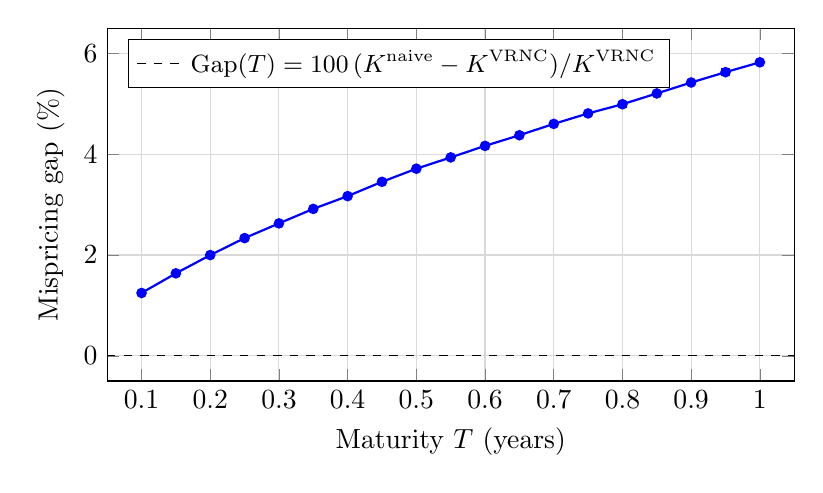
\begin{tikzpicture}
\begin{axis}[
    width=0.85\textwidth,
    height=0.5\textwidth,
    xlabel={Maturity $T$ (years)},
    ylabel={Mispricing gap (\%)},
    xmin=0.05, xmax=1.05,
    ymin=-0.5, ymax=6.5,
    grid=major,
    grid style={gray!30},
    legend pos=north west,
    legend style={font=\small},
]

% Zero reference line
\addplot[black, thin, dashed] coordinates {(0.05, 0) (1.05, 0)};

% Mispricing gap with error bars
\addplot[thick, blue, mark=*, mark size=1.5pt,
    error bars/.cd, y dir=both, y explicit]
    coordinates {
  (0.10, 1.247) +- (0, 0.019)
  (0.15, 1.637) +- (0, 0.022)
  (0.20, 1.999) +- (0, 0.023)
  (0.25, 2.336) +- (0, 0.029)
  (0.30, 2.628) +- (0, 0.026)
  (0.35, 2.916) +- (0, 0.031)
  (0.40, 3.169) +- (0, 0.033)
  (0.45, 3.453) +- (0, 0.043)
  (0.50, 3.713) +- (0, 0.044)
  (0.55, 3.937) +- (0, 0.045)
  (0.60, 4.166) +- (0, 0.045)
  (0.65, 4.377) +- (0, 0.050)
  (0.70, 4.602) +- (0, 0.052)
  (0.75, 4.810) +- (0, 0.051)
  (0.80, 4.992) +- (0, 0.054)
  (0.85, 5.206) +- (0, 0.057)
  (0.90, 5.423) +- (0, 0.058)
  (0.95, 5.628) +- (0, 0.062)
  (1.00, 5.824) +- (0, 0.063)
};
\addlegendentry{$\mathrm{Gap}(T) = 100\,(K^{\mathrm{naive}} - K^{\mathrm{VRNC}})/K^{\mathrm{VRNC}}$}

\end{axis}
\end{tikzpicture}
\caption{Mispricing gap for variance swap strikes under a local (pointwise)
risk-neutral specification versus the Volterra risk-neutral constraint (VRNC).
$H = 0.1$, $\rho = -0.7$, 100{,}000 paths; error bars show bootstrap standard error.
The gap increases with maturity, reflecting memory-induced drift terms that are
invisible to local drift cancellation.}
\label{fig:mispricing-gap}
\end{figure}

\begin{proposition}[Variance swap drift dichotomy]\label{prop:var-swap-drift}
Let $V_t(T) := \E^{\QQ}[\int_t^T \sigma_s^2\,ds \mid \F_t]$ denote the forward
variance process. Under a local (pointwise) risk-neutral specification
$\QQ_{\mathrm{local}}$, the predictable finite-variation component in the
Doob--Meyer decomposition of $V_t(T)$ includes a memory-driven term proportional
to $\int_0^t K(t,s)\,ds$. Under the VRNC \eqref{eq:rn-constraint}, this
predictable drift vanishes at the level of the forward variance process.
\end{proposition}

This dichotomy reveals a \textbf{selection principle}: even after martingale
pricing of the underlying is enforced, variance-linked claims can remain
underdetermined unless an additional memory-consistency constraint (the VRNC)
is imposed. Multiple equivalent martingale measures may coexist, but only
those satisfying the VRNC correctly price variance-linked claims.

\textbf{Mathematical contrast.} Under the two specifications, the expected
integrated variance differs by a memory-driven residual:
\[
\E^{\QQ_{\text{local}}}\!\left[\int_0^T \sigma_t^2\,dt\right]
= \E^{\QQ_{\text{VRNC}}}\!\left[\int_0^T \sigma_t^2\,dt\right]
+ \int_0^T \text{(residual memory term)}_t\,dt.
\]
The VRNC forces this residual to have zero predictable drift under
$\QQ_{\text{VRNC}}$. The discrepancy is structural and persists across
parameter choices; it reflects the memory structure of the model, not
calibration artifacts.

\textbf{Interpretation.} In models with memory, risk-neutrality is not merely a
local drift cancellation condition; it is a Volterra-type constraint (the VRNC)
ensuring the correct pricing of variance-linked claims. The naive approach
satisfies price martingality but violates the deeper constraint. This explains
why calibration to vanilla options (which depend on marginals, hence bracket
geometry) can succeed while hedging variance-dependent claims fails: the two
tasks impose structurally different constraints.

\subsubsection{Summary of Monte Carlo validation}

Table~\ref{tab:mc-summary} summarizes all stochastic claims.

\begin{table}[h]
\centering
\caption{Monte Carlo validation summary (50{,}000--100{,}000 paths per test).}
\label{tab:mc-summary}
\begin{tabular}{lp{5.5cm}c}
\hline
\textbf{Test} & \textbf{Criterion} & \textbf{Result} \\
\hline
$Z^{\QQ}$ martingale & $\E[Z^{\QQ}_T - Z^{\QQ}_t] \approx 0$ & Pass ($|z| < 0.2$) \\
Decomposition & $Z = Z^{\QQ} + B^\theta$ pathwise & Pass (error $< 10^{-3}$) \\
Discounted $S$ martingale & $\E^{\QQ}[S_t/B_t] = S_0$ for all $t$ & Pass ($|z| < 1.3$) \\
Naive vs.\ operator $\theta$ & Operator gap $<$ naive gap & Pass (0.9\% vs 3.6\%) \\
Variance swap pricing & VRNC reduces naive gap & Pass (2--6\% gap corrected) \\
Importance sampling & Direct $=$ reweighted & Pass ($< 0.5\%$ diff) \\
Covariance preservation & Simulated $\approx$ theoretical & Pass ($< 1.5\%$ error) \\
Rough kernel ($H = 0.3$) & $\dGamma$ scaling extracts $H$ & Pass (exact) \\
\hline
\end{tabular}
\end{table}

%==============================================================================
\section{Scope and Limitations}\label{sec:limitations}
%==============================================================================

\subsection{What this paper provides}

\begin{enumerate}
\item An explicit measure-change framework for Volterra processes that requires no
semimartingale assumption on the observable.
\item The bracket invariance principle: geometric features are measure-independent.
\item The risk-neutral constraint as an operator equation: actionable for
calibration in memory markets.
\item Density calculus machinery for computing hedging strategies under $\QQ$.
\end{enumerate}

\subsection{What this paper does not provide}

\begin{enumerate}
\item \textbf{Pathwise theory:} We work in $L^2$, not pathwise. Rough path
Girsanov theory requires different machinery.
\item \textbf{Existence/uniqueness for the Volterra equation:} We show the
risk-neutral constraint is a Volterra equation; solving it in full generality
requires case-by-case analysis.
\item \textbf{Jump processes:} The exponential Girsanov form \eqref{eq:doleans}
is for continuous martingales. L\'evy or Poisson drivers require the
jump-compensator version, though the ``driver-level then operator pushforward''
philosophy extends naturally.
\end{enumerate}

%==============================================================================
\section{Conclusion}\label{sec:conclusion}
%==============================================================================

We have developed Girsanov theory for Volterra processes, establishing:

\begin{enumerate}
\item The measure change acts at the driver level, inducing an operator-valued
drift on observables (\Cref{thm:girsanov-main}).

\item The fresh-noise energy $\dGamma(t,h)$ is invariant under equivalent
measure changes---it is a geometric quantity, not a probabilistic one
(\Cref{thm:girsanov-main}(3)).

\item Risk-neutral pricing in memory markets requires solving a Volterra
equation for the market price of risk (\Cref{cor:rn-constraint}).

\item The Clark--Ocone--type representation under $\QQ$ provides the hedging
density, computable via Bayes' formula and the modified Leibniz rule
(\Cref{thm:clark-ocone-Q}).
\end{enumerate}

The bracket invariance principle is the conceptual core: \emph{equivalent
measure changes preserve the Volterra bracket geometry and induce only
operator-valued drift shifts on kernel observables}.

%==============================================================================
\section*{Acknowledgments}
%==============================================================================

The author works in financial risk management; the risk-neutral pricing
application arose from practical experience with memory models. AI tools
were used as interactive assistants for mathematical exploration. The
author is responsible for all content.

%==============================================================================
% References
%==============================================================================

\begin{thebibliography}{99}

\bibitem{Fontes2026a}
R.~Fontes.
\newblock Stochastic calculus as operator factorization.
\newblock \emph{arXiv:2601.09976}, 2026.

\bibitem{Fontes2026b}
R.~Fontes.
\newblock Stochastic calculus for rough fractional {B}rownian motion via
operator factorization.
\newblock \emph{arXiv:2601.09967}, 2026.

\bibitem{Fontes2026c}
R.~Fontes.
\newblock An {I}t\^o formula via predictable projection for non-semimartingale
processes.
\newblock \emph{arXiv:2601.10359}, 2026.

\bibitem{Fontes2026d}
R.~Fontes.
\newblock The operator derivative: Intrinsic properties, structural conditions,
and process-dependent extensions.
\newblock \emph{Preprint}, 2026.

\bibitem{Fontes2026e}
R.~Fontes.
\newblock {PDE} generators from energy space structure in {F}eynman--{K}ac theory.
\newblock \emph{Preprint}, 2026.

\bibitem{Fontes2026f}
R.~Fontes.
\newblock Volterra representations and operator brackets: The kernel-level
geometry of non-{M}arkovian calculus.
\newblock \emph{Preprint}, 2026.

\bibitem{Fontes2026g}
R.~Fontes.
\newblock Bracket-corrected differentiation for kernel-driven processes:
Why stochastic calculus rules deform, and what it means for hedging.
\newblock \emph{Preprint}, 2026.

\bibitem{KaratzasShreve1991}
I.~Karatzas and S.~E. Shreve.
\newblock \emph{Brownian Motion and Stochastic Calculus}.
\newblock Springer, second edition, 1991.

\bibitem{JacodShiryaev2003}
J.~Jacod and A.~N. Shiryaev.
\newblock \emph{Limit Theorems for Stochastic Processes}.
\newblock Springer, second edition, 2003.

\bibitem{LiptserShiryayev2001}
R.~S. Liptser and A.~N. Shiryayev.
\newblock \emph{Statistics of Random Processes I: General Theory}.
\newblock Springer, second edition, 2001.

\bibitem{Protter2005}
P.~E. Protter.
\newblock \emph{Stochastic Integration and Differential Equations}.
\newblock Springer, second edition, 2005.

\bibitem{Decreusefond1999}
L.~Decreusefond and A.~S. \"Ust\"unel.
\newblock Stochastic analysis of the fractional {B}rownian motion.
\newblock \emph{Potential Analysis}, 10(2):177--214, 1999.

\bibitem{FrizHairer2014}
P.~K. Friz and M.~Hairer.
\newblock \emph{A Course on Rough Paths}.
\newblock Springer, 2014.

\bibitem{GatheralJaissonRosenbaum2018}
J.~Gatheral, T.~Jaisson, and M.~Rosenbaum.
\newblock Volatility is rough.
\newblock \emph{Quantitative Finance}, 18(6):933--949, 2018.

\bibitem{Nualart2006}
D.~Nualart.
\newblock \emph{The {M}alliavin Calculus and Related Topics}.
\newblock Springer, second edition, 2006.

\end{thebibliography}

\end{document}
